\documentclass[12pt,letterpaper]{exam}
\usepackage[lmargin=1in,rmargin=1in,tmargin=1in,bmargin=1in]{geometry}
\usepackage{../style/exams}

% -------------------
% Course & Exam Information
% -------------------
\newcommand{\course}{MAT 100: Exam 1}
\newcommand{\term}{Fall -- 2023}
\newcommand{\examdate}{10/11/2023}
\newcommand{\timelimit}{85 Minutes}

\setbool{hideans}{true} % Student: True; Instructor: False

% -------------------
% Content
% -------------------
\begin{document}

\examtitle
\instructions{Write your name on the appropriate line on the exam cover sheet. This exam contains \numpages\ pages (including this cover page) and \numquestions\ questions. Check that you have every page of the exam. Answer the questions in the spaces provided on the question sheets. Be sure to answer every part of each question and show all your work. If you run out of room for an answer, continue on the back of the page --- being sure to indicate the problem number.} 
\scores
\bottomline
\newpage

% ---------
% Questions
% ---------
\begin{questions}

% Question 1
\newpage
\question[10] You have been saving for a new laptop and printer. You will finally have enough money to purchase them both next month. The laptop costs \$1,899 and the printer costs \$220. Next month, the laptop will go on sale for 5\% less while the printer will be marked up 4\%. The sales tax on the items is 7\%. When you make the purchase of the laptop and printer next month, how much will you pay in total?



% Question 2
\newpage
\question[10] A home was purchased for \$350,000. Unfortunately, home values in the region have depreciated by 1\% per year, every year, for the last 20~years. What is the value of the home now? 



% Question 3
\newpage
\question[10] It is the end of the semester and a teacher is computing a student's average. Each grading component, the components weight in the course average, and the students grade in that component is given below. What is the student's course average? \par
	\begin{table}[H]
	\centering
	\begin{tabular}{lcc}
	Grade Component & Component Value & Student Grade \\ \hline
	Homework & 40\% & 72\% \\
	Attendance & \phantom{0}5\% & 90\% \\
	Midterm & 10\% & 82\% \\
	Final & 20\% & 88\% \\
	Project & 25\% & 92\%
	\end{tabular}
	\end{table}



% Question 4
\newpage
\question[10] Showing all your work, perform the following unit conversions:
	\begin{enumerate}[(a)]
	\item 2~quarts to liters [1~quart = 4~cups; 1~cup = 8~fl oz; 29.57~ml = 1~fl oz]
	\item 1,500 square feet to m$^2$ [0.3048~m = 1~ft]
	\item 9.8~m/s$^2$ to feet per square minute [1~m = 3.28084~ft]
	\end{enumerate}



% Question 5
\newpage
\question[10] A strange escape room has a design layout that is given below. The ceiling height for the room is 8~ft. Find the perimeter, area, and volume of this room.
	\[
	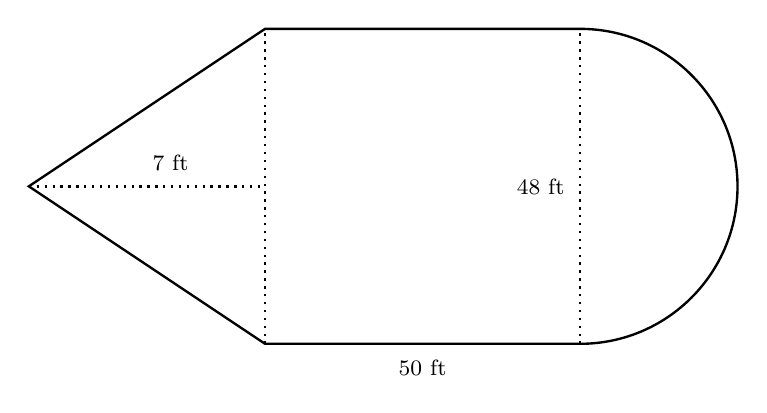
\begin{tikzpicture}
	\draw[line width=0.03cm] (4,-2) -- (0,-2) -- (-3,0) -- (0,2) -- (4,2);
	\draw[line width=0.03cm] (4,-2) arc(-90:90:2);
	
	\draw[line width=0.03cm,dotted] (-3,0) -- (0,0);
	\draw[line width=0.03cm,dotted] (0,-2) -- (0,2);
	\draw[line width=0.03cm,dotted] (4,-2) -- (4,2);
	
	\node at (-1.2,0.3) {\footnotesize 7~ft};
	\node at (2,-2.3) {\footnotesize 50~ft};
	\node at (3.5,0) {\footnotesize 48~ft};
	\end{tikzpicture}
	\]   



% Question 6
\newpage
\question[10] Explain why $f(x, y)= x^2 - y + 3$ is a function and find the value of $f$ at $(x, y)= (-1, 5)$. 



% Question 7
\newpage
\question[10] Consider the function $f(x)= 9 - 2x$. 
	\begin{enumerate}[(a)]
	\item Explain why $f(x)$ is a linear function. 
	\item Find the slope and $y$-intercept for $f(x)$. 
	\item Find the $x$-intercept for $f(x)$. 
	\item Find $f(3)$. 
	\item Find an $x$ such that $f(x)= 5$. 
	\end{enumerate}
	


% Question 8
\newpage
\question[10] Find the linear function through the points $(-1, 6)$ and $(3, -4)$. Is this linear function increasing or decreasing? Explain. 



% Question 9
\newpage
\question[10] You keep a secret lunchbox under your bed filled with cash. The lunchbox currently contains \$2,500. Each week, you place \$80 into the lunchbox. Let $M(w)$ denote the amount of money in the lunchbox $w$~weeks from now. 
	\begin{enumerate}[(a)]
	\item Explain why $M(w)$ is linear.
	\item Find $M(w)$. 
	\item Use (b) to find how long until the lunchbox has \$10,000. 
	\end{enumerate}



% Question 10
\newpage
\question[10] You and a coworker are responsible for maintaining a portion of a golf course. You can weed the field in 8~hours. When your coworker helps you, you are able to do it in 5~hours. How fast can your coworker weed the field?


\end{questions}
\end{document}